Considérons que nous cherchons de manière empirique à obtenir des connaissances sur l'aire de base et le volume des formes géométriques tridimensionelles \marginnote{Le code de cet exemple est disponible\url{https://github.com/mathieulagrange/expLanes/tree/master/demo/geometricShape}}.

La création de l'expérimentation \textsl{geometricShape} se fait comme suit :
\begin{lstlisting}
expCreate('geometricShape');
\end{lstlisting}
Nous pouvons ensuite instantier deux étapes de traitement, une qui se chargera du calcul de l'aire de la base:
\begin{lstlisting}
geometricShape('addStep', 'base');
\end{lstlisting}
et une autre du volume :
\begin{lstlisting}
geometricShape('addStep', 'space');
\end{lstlisting}
Nous nous intéressons dans cette expérimentation à l'influence potentielle des différents attributs (forme, couleur, rayon, largeur, hauteur) sur l'aire de sa base et son volume. Nous considérons donc chacun de ces attributs comme des facteur expérimentaux avec des modalités données.

Les formes étudiées sont le cylindre, la pyramide et le cube, nous ajoutons donc un facteur nommé \mcode{'shape'} de trois modalités :
\begin{lstlisting}
geometricShape('addFactor', ...
	{'shape', {'cylinder', 'pyramid', 'cube'}});
\end{lstlisting}
La couleur peut être bleu ou rouge, le rayon peut être de 2, 4, ou 6 mètres, la largeur de la pyramide et du cube peut être de 1, 2, et 3 mètres et la hauteur de 2, 4 ,et 6 mètres. On note ici que certains facteurs ne devront être explorés que pour une modalité d'un autre facteur. Il est en pratique très utile de pouvoir exprimer ce type d'exclusion, qui est courante dans tout plan expérimental de complexité raisonnable avec plusieurs approches mises en compétition. Le fichier statique, nommé \mcode{geshFactors.txt} pour cette expérimentation, permet de stocker les informations nécessaires à la création du plan expérimental est de cette forme  :
\begin{lstlisting}
Factors:
1    shape =  =  = {'cylinder', 'pyramid', 'cube'}
2    color =  =  = {'blue', 'red'}
3    radius =  = 1/1 = [2, 4, 6]
4    width =  = 1/[2 3] = 1:3
5    height = 2 = 1/[1 2] = 2:2:6
\end{lstlisting}
La ligne 5 peut se lire comme suit, le facteur \mcode{'height'} n'est pertinent que pour l'étape de traitement 2 et les modalités 1 et 2 du facteur 1.

Les deux étapes de traitement sont implantées comme suit. Chaque étape dispose de la même signature, la variable \textsl{config} expose la configuration de l'expérimentation, la variable \textsl{setting} la condition expérimentale courante, et la variable \textsl{data} expose les données produite par l'étape précédente ou les données d'entrée pour la première étape.

La première étape se charge du calcul de l'aire de la base de la forme géométrique. Pour les besoins de l'exemple, on suppose ici que $/pi$ n'est pas connu de manière précise, ce qui est simulé ici par l'ajout d'une certaine incertitude sur sa mesure :

\begin{lstlisting}
function [config, store, obs] = gesh1base(config, setting, data)

uncertainty = randn(1, 100);
switch setting.shape
    case 'cylinder'
        baseArea = (pi+uncertainty)*setting.radius^2;
    otherwise
        baseArea  = setting.width^2;
end
store.baseArea = baseArea;
obs.area = baseArea;
\end{lstlisting}

La seconde étape complète le calcul effectué par la première pour calculer le volume de la forme géométrique :
\begin{lstlisting}
function [config, store, obs] = gesh2space(config, setting, data)

switch setting.shape
    case 'cube'
       volume = data.baseArea*setting.width;
    case 'cylinder'
        volume = data.baseArea*setting.height;
    case 'pyramid'
        volume = data.baseArea*setting.height/3;
end

obs.baseArea = data.baseArea;
obs.volume = volume;
\end{lstlisting}

\begin{marginfigure}
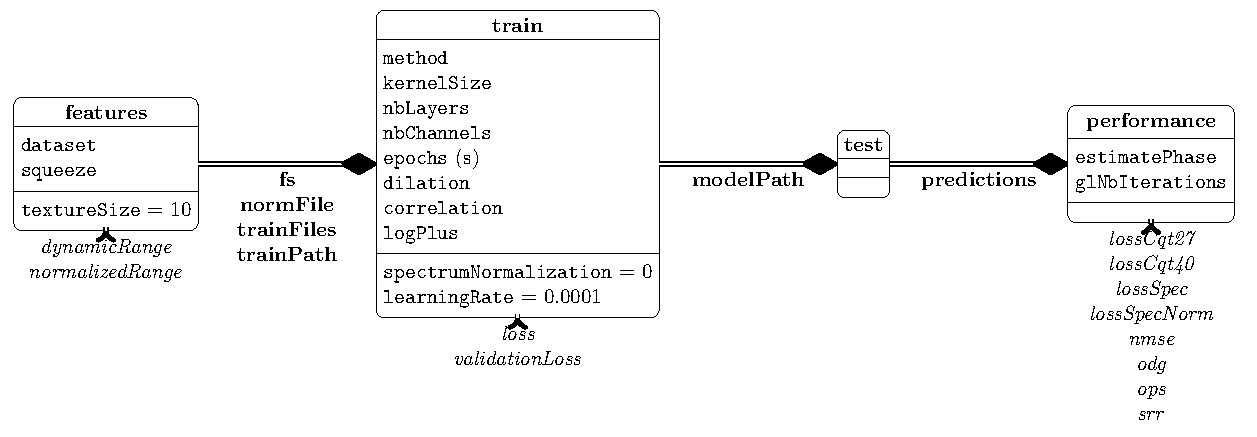
\includegraphics[width=\textwidth]{factors}
La commande \mcode{geometricShape('f')} génère un diagramme où les éléments principaux de l'expérimentation sont visibles (étapes de traitement, facteurs, données sauvegardées, observations).
\end{marginfigure}

Une fois l'implantation effectuée, le traitement est effectué avec la commande \mcode{'do'}. Par exemple, la commande
\begin{lstlisting}
geometricShape('do', 1);
\end{lstlisting}
demande le calcul de l'étape 1 pour toutes les conditions expérimentales (qui sont au nombre de 18). Il est souvent nécessaire de ne pas effectuer le plan expérimental complet (étude spécifique, reprise sur erreur, ...), le mécanisme de masquage est alors utilisé. Par exemple, la commande
\begin{lstlisting}
geometricShape('do', 0, 'mask', {[1 2] 0 1})}
\end{lstlisting}
demande le calcul successif des deux étapes pour les cylindres de rayon 2 et toutes les pyramides.

Après le traitement des deux étapes, le répertoire dédié au stockage des données de calcul et d'observations contient : \\
\begin{Verbatim}[fontsize=\scriptsize]
	base/color: blue, radius: 2, shape: cylinder_data.mat            space/color: blue, height: 2, shape: pyramid, width: 2_obs.mat
	base/color: blue, radius: 2, shape: cylinder_obs.mat             space/color: blue, height: 2, shape: pyramid, width: 3_obs.mat
	base/color: blue, radius: 4, shape: cylinder_data.mat            space/color: blue, height: 4, radius: 2, shape: cylinder_obs.mat
	base/color: blue, radius: 4, shape: cylinder_obs.mat             space/color: blue, height: 4, radius: 4, shape: cylinder_obs.mat
	base/color: blue, radius: 6, shape: cylinder_data.mat            space/color: blue, height: 4, radius: 6, shape: cylinder_obs.mat
	base/color: blue, radius: 6, shape: cylinder_obs.mat             space/color: blue, height: 4, shape: pyramid, width: 1_obs.mat
	base/color: blue, shape: cube, width: 1_data.mat                 space/color: blue, height: 4, shape: pyramid, width: 2_obs.mat
	base/color: blue, shape: cube, width: 1_obs.mat                  space/color: blue, height: 4, shape: pyramid, width: 3_obs.mat
	...							      ...
\end{Verbatim}

Ce n'est pas explicite dans cet exemple, mais les fichiers \mcode{\_data} dédiés au stockage des données de calculs sont souvent de taille plus conséquente que les observations qui elles ont vocation à rester de taille raisonnable pour pouvoir être transférées des machines de calcul aux machines de développement et de visualisation pour pouvoir être aisément analysées. Pour toute expérimentation de taille raisonnable, les noms de fichiers peuvent être compactés pour ne pas dépasser les 250 caractères requis par la plupart des systèmes de gestions de fichiers.

\`A la fin du traitement, les observations de la dernière étape de traitement sont affichées :
\begin{Verbatim}[fontsize=\scriptsize]
	Loaded data files dates are in the range: | 01-Apr-2019 10:15:55 || 01-Apr-2019 10:15:56 |
	    'shape'       'color'    'radius'    'width'    'height'    'baseArea'          'time'    'volume'
	    '---'         '---'      '---'       '---'      '---'       '---'               '---'     '---'
	    'cylinder'    'blue'     '2'         ''         '2'         '  12.55 (4.32)'    '0.22'    '   25.11 (8.63)'
	    'cylinder'    'blue'     '2'         ''         '4'         '  12.55 (4.32)'    '0.09'    '  50.22 (17.27)'
	    'cylinder'    'blue'     '2'         ''         '6'         '  12.55 (4.32)'    '0.00'    '  75.32 (25.90)'
	    'cylinder'    'blue'     '4'         ''         '2'         ' 50.85 (16.54)'    '0.00'    ' 101.70 (33.08)'
	    'cylinder'    'blue'     '4'         ''         '4'         ' 50.85 (16.54)'    '0.00'    ' 203.41 (66.15)'
	    'cylinder'    'blue'     '4'         ''         '6'         ' 50.85 (16.54)'    '0.00'    ' 305.11 (99.23)'
	    'cylinder'    'blue'     '6'         ''         '2'         '109.79 (33.75)'    '0.00'    ' 219.57 (67.50)'
	    'cylinder'    'blue'     '6'         ''         '4'         '109.79 (33.75)'    '0.01'    '439.14 (135.00)'
	    'cylinder'    'blue'     '6'         ''         '6'         '109.79 (33.75)'    '0.00'    '658.72 (202.50)'
	    'cylinder'    'red'      '2'         ''         '2'         '  11.92 (4.33)'    '0.00'    '   23.84 (8.66)'
	    'cylinder'    'red'      '2'         ''         '4'         '  11.92 (4.33)'    '0.00'    '  47.68 (17.32)'
\end{Verbatim}

L'accès à une grande diversité de mises en forme de l'exposition des observations utiles au discours est un élément nécessaire pour une expérimentation efficace. La plateforme \explanes dispose d'un grand nombre de fonctionalités conçues pour permettre une certaine flexibilité dans leurs usages.

Par exemple, ce dernier affichage peut être ré-obtenu grâce à la commande suivante :
\begin{lstlisting}
geometricShape('display', 2, 'expose', '>', 'mask', {[1 2] 0 1});
\end{lstlisting}
La commande :
\begin{lstlisting}
geometricShape('display', 2, 'mask', {1 0 1},...
 'expose', {'t', 'obs', 2});
\end{lstlisting}
affiche les volumes (observations 2) de l'étape 2 pour chaque cylindre de rayon 2 triés par la première observation sélectionnée. La fonte rouge indique la plus haute valeur, et les valeurs en gras, celles qui ne sont pas statistiquement différentes, au sens d'un t-test par paires effectué entre les observations de la condition expérimentale et celle correspondant à la plus haute valeur.

\begin{margintable}
\caption{Visualisation sous forme de table \LaTeX.}
\begin{tabular}{llc}
color & height & volume \\
\hline
blue & 2 &  26.12$\pm$9.30 \\
blue & 4 & 52.23$\pm$18.60 \\
blue & 6 & \textbf{\textcolor{red}{78.35$\pm$27.90}} \\
red & 2 &  24.61$\pm$7.54 \\
red & 4 & 49.23$\pm$15.07 \\
red & 6 & \textbf{73.84$\pm$22.61} \\
\end{tabular}
\end{margintable}

Dans notre exemple, même si le cylindre bleu est plus volumineux que le rouge, cette différence n'étant pas significative, on peut en conclure expérimentalement que la couleur n'influe pas sur le volume. Une fois la phase d'analyse des résultats effectuée, nous pouvons alors communiquer les résultats grâce à la production de rapports d'expérimentation. Quelques exemples de rapports d'expérimentation pour des expérimentations plus ambitieuses sont disponibles sur le site du projet \textsl{expLanes}.
